\documentclass{article}
\usepackage{bm}
\usepackage{amssymb}
\usepackage{amsmath}
\usepackage{tikz}
\usepackage{url}
\usetikzlibrary{positioning}

\title{Basic MLP with manually-derived Backprop}
\author{Teo Asinari}
\date{\today}

\begin{document}
\maketitle

\section{Introduction}
\paragraph{Goal:} To design, train and use a simple 3-layer MLP for binary classification
of size-2 vectors.
\paragraph{Design:} of the form \[[(layer\_size, Activation)...]\]: [(2, ReLU), (2, ReLU), (1, Sigmoid)]
\subsection{Diagrams}
\subsubsection{Vectorized Diagram (Equiv to Roger Grosse' 'Computational Graph')}
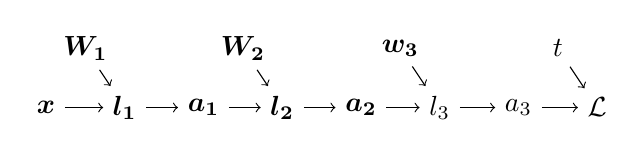
\begin{tikzpicture}[]
    \node (input) at (1,1) {$\bm{x}$};
    \node (weight1) at (1.5,1.75) {$\bm{W_1}$};
    \node (inputLayer) at (2,1) {$\bm{l_1}$};
    \node (activation1) at (3,1) {$\bm{a_1}$};
    \node (hiddenLayer) at (4,1) {$\bm{l_2}$};
    \node (weight2) at (3.5,1.75) {$\bm{W_2}$};
    \node (activation2) at (5,1) {$\bm{a_2}$};
    \node (outputLayer) at (6,1) {$l_3$};
    \node (weight3) at (5.5,1.75) {$\bm{w_3}$};
    \node (activation3) at (7,1) {$a_3$};
    \node (target) at (7.5,1.75) {$t$};
    \node (loss) at (8,1) {$\mathcal{L}$};


\draw[->] (input) -- (inputLayer);
\draw[->] (weight1) -- (inputLayer);
\draw[->] (inputLayer) -- (activation1);
\draw[->] (activation1) -- (hiddenLayer);
\draw[->] (weight2) -- (hiddenLayer);
\draw[->] (hiddenLayer) -- (activation2);
\draw[->] (activation2) -- (outputLayer);
\draw[->] (weight3) -- (outputLayer);
\draw[->] (outputLayer) -- (activation3);
\draw[->] (target) -- (loss);
\draw[->] (activation3) -- (loss);

\end{tikzpicture}
\subsubsection{Expanded Diagram (Equiv. to Roger Grosse' 'Network Architecture')}
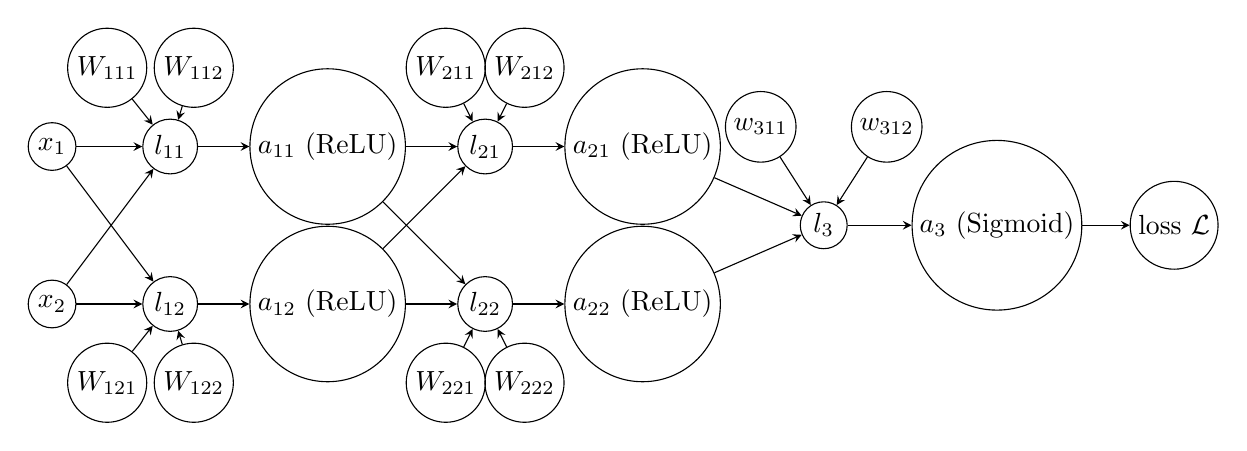
\begin{tikzpicture}[%
    activation/.style={%
        draw,
        circle,
        inner sep=2pt,
        minimum size=0.5cm,
        node distance=0.5cm
    },
    input/.style={%
        draw,
        circle,
        inner sep=2pt,
        minimum size=0.5cm,
        node distance=0.5cm
    },
    weight/.style={%
        draw,
        circle,
        inner sep=2pt,
        minimum size=0.5cm,
        node distance=0.5cm
    },
    inputLayer/.style={%
        draw,
        circle,
        inner sep=2pt,
        minimum size=0.5cm,
        node distance=0.5cm
    },
    hidden/.style={%
        draw,
        circle,
        inner sep=2pt,
        minimum size=0.5cm,
        node distance=0.5cm
    },
    output/.style={%
        draw,
        circle,
        inner sep=2pt,
        minimum size=0.5cm,
        node distance=0.5cm
    },
    >=stealth
]

% Inputs
    \node[input] (input1) at (1,1) {$x_1$};
    \node[input] (input2) at (1,-1) {$x_2$};

% Input layer 1 (L_1)
    \node[inputLayer] (inputLayer1) at (2.5,1) {$l_{11}$};
    \node[inputLayer] (inputLayer2) at (2.5, -1) {$l_{12}$};
    \node[weight] (weight111) at (1.7, 2) {$W_{111}$};
    \node[weight] (weight112) at (2.8, 2) {$W_{112}$};
    \node[weight] (weight121) at (1.7, -2) {$W_{121}$};
    \node[weight] (weight122) at (2.8, -2) {$W_{122}$};

% Input Layer Activation
    \node[activation] (activation11) at (4.5, 1) {$a_{11}$ (ReLU)};
    \node[activation] (activation12) at (4.5, -1) {$a_{12}$ (ReLU)};

% Hidden layer 2 (L_2)
    \node[hidden] (hidden1) at (6.5, 1) {$l_{21}$};
    \node[hidden] (hidden2) at (6.5, -1) {$l_{22}$};
    \node[weight] (weight211) at (6, 2) {$W_{211}$};
    \node[weight] (weight212) at (7, 2) {$W_{212}$};
    \node[weight] (weight221) at (6, -2) {$W_{221}$};
    \node[weight] (weight222) at (7, -2) {$W_{222}$};

%

% Hidden Layer Activation
    \node[activation] (activation21) at (8.5, 1) {$a_{21}$ (ReLU)};
    \node[activation] (activation22) at (8.5, -1) {$a_{22}$ (ReLU)};
% Output layer (L_3)
    \node[output] (output1) at (10.8, 0) {$l_{3}$};
    \node[weight] (weight311) at (10, 1.25) {$w_{311}$};
    \node[weight] (weight312) at (11.6, 1.25) {$w_{312}$};

% Output Layer activation
    \node[activation] (activation3) at (13, 0) {$a_{3}$ (Sigmoid)};

% Loss
    \node[output] (loss) at (15.25, 0) {loss $\mathcal{L}$};

% Arrows
\draw[->] (input1) -- (inputLayer1);
\draw[->] (input1) -- (inputLayer2);
\draw[->] (input2) -- (inputLayer1);
\draw[->] (input2) -- (inputLayer2);


\draw[->] (weight111) -- (inputLayer1);
\draw[->] (weight112) -- (inputLayer1);
\draw[->] (weight121) -- (inputLayer2);
\draw[->] (weight122) -- (inputLayer2);

\draw[->] (inputLayer1) -- (activation11);
\draw[->] (inputLayer2) -- (activation12);

\draw[->] (activation11) -- (hidden1);
\draw[->] (activation11) -- (hidden2);
\draw[->] (activation12) -- (hidden1);
\draw[->] (activation12) -- (hidden2);

\draw[->] (weight211) -- (hidden1);
\draw[->] (weight212) -- (hidden1);
\draw[->] (weight221) -- (hidden2);
\draw[->] (weight222) -- (hidden2);


\draw[->] (hidden1) -- (activation21);
\draw[->] (hidden2) -- (activation22);

\draw[->] (activation21) -- (output1);
\draw[->] (activation22) -- (output1);

\draw[->] (output1) -- (activation3);


\draw[->] (weight311) -- (output1);
\draw[->] (weight312) -- (output1);


\draw[->] (activation3) -- (loss);

\end{tikzpicture}

\subsection{Definitions}
\subsubsection{Remark on general notation}
Since it seems that mathematical notation in this field tends to suffer from overloading, imprecision/lack of specificity, a lack of convention, poor readability, and a generally poor aesthetic/deisgn sense, I am going to try to avoid worsening the situation. So, for the purpose of this work, 
all non-bold variables denote scalars. A bold lower-case variable denotes a vector, a bold upper-case a Matrix. 
A non-bold lower-case may denotes either an arbitrary scalar variable or if subscripted typically an element of a vector.
A non-bold upper-case, if subscripted, will typically denote a matrix element.
\subsubsection{Remark on weight notation}
$w_{i,j,k}$ is to say the weight at the $i$-th layer, $j$-th neuron, $k$-th weight.
Hence $w_{111}$ is the first weight of the first neuron in the first layer, etc.
\subsubsection{Remark on layer notation}
This is a sub-case of the weight notation. I.e., $L_{ij}$ is the scalar value of the $j$-th neuron at the $i$-th layer, etc.
\subsubsection{Neuron firing calculation} This is just a straightforward dot-product. We have:
\[l_{ij}=\bm{W}_{ij}\bm{x}_i \]
Where $\bm{x}_i$ in this case is referring to a more general notion of 'layer input', not necessarily just the first input to the network as in the diagrams above.
\subsection{BackPropagation Derivation}
\paragraph{Notation for derivative of loss w.r.t. to a function} I will be using the following: $\overline{f} = \frac{\partial{\mathcal{L}}}{\partial{f}}$. This notation was introduced by Roger Grosse from the University of Toronto.
\paragraph{Pa(x) and Ch(x)} these refer to the sets of parent and child vertices of a vertex in a graph.
\paragraph{General Approach} Let's label the computational graph nodes as $v_1,...,v_N$ with some topological ordering. 
Then, our general goal for backprop is to compute $\overline{v_i}$ for $i \in {1,...N}$. With these, we can trivially calculate the weight updates.
We compute a forward pass of the network, then set $v_N=1$, then, for $i=N-1, ... , 1$, we have:
\begin{equation}
    \overline{v_i} = \sum_{j \in \text{Ch}(v_i)} \overline{v_j} \frac{\partial{v_j}}{\partial{v_i}} \quad  \text{(The Backprop Rule)}
\end{equation}
\subsubsection{Applying the backprop rule}
\paragraph{Loss and final activation}
Then, going backwards through the 'computational graph', starting at the end:
\begin{equation}\overline{\mathcal{L}} = 1\end{equation}
\[\overline{a_3} = \overline{\mathcal{L}} \frac{\partial{\mathcal{L}}}{\partial{a_3}}\]
\[\overline{a_3} = (1) \frac{\partial{\mathcal{L}}}{\partial{a_3}}\]
\[\overline{a_3} = \frac{\partial{\mathcal{L}}}{\partial{a_3}}\]
\[\overline{a_3} = \frac{\partial}{\partial{a_3}} \frac{1}{2}(a_3 - t)^{2}\]
\[\overline{a_3} = (a_3 - t) \frac{\partial}{\partial{a_3}} (a_3 - t)\]
\[\overline{a_3} = (a_3 - t) (1)\]
\begin{equation}
\overline{a_3} = (a_3 - t)
\end{equation}
\paragraph{Final layer}
$\bm{N.B.}$ I use $\sigma$ to denote the sigmoid function here, not an activation function.
\[\overline{l_3} = \overline{a_3} \frac{\partial{a_3}}{\partial{l_3}}\]
\[\overline{l_3} = \overline{a_3} \frac{\partial}{\partial{l_3}} \sigma(l_3)\]
\begin{equation}
    \overline{l_3} = \overline{a_3} \hspace{0.125cm} \sigma(l_3) (1 - \sigma(l_3))
\end{equation}
\paragraph{Final layer weights}
\[\overline{w_{31i}} = \overline{l_3} \frac{\partial}{\partial{w_{31i}}} l_3\]
\[\overline{w_{31i}} = \overline{l_3} \frac{\partial}{\partial{w_{31i}}} \sum_{j} w_{31j} a_{2j}\]
\begin{equation}
    \overline{w_{31i}} = \overline{l_3} a_{2i}
\end{equation}
\paragraph{Second layer activation}
\[\overline{a_{2i}} = \overline{l_3} \frac{\partial}{\partial{a_{2i}}} l_3\]
\[\overline{a_{2i}} = \overline{l_3} \frac{\partial}{\partial{a_{2i}}} \sum_{j} w_{31j}a_{2j}\]
\begin{equation}
    \overline{a_{2i}} = \overline{l_3} w_{31i}
\end{equation}
\paragraph{Second layer}
\[\overline{l_{2i}} = \overline{a_{2i}} \frac{\partial}{\partial{l_{2i}}} a_{2i} \]
\[\overline{l_{2i}} = \overline{a_{2i}} \frac{\partial}{\partial{l_{2i}}}\text{ReLU}(l_{2i}) \]
Note that $d/dx($ReLU$(x))$ is the heaviside step function $\theta (x)$: 
\[
\begin{cases}
    1 & \text{if } x > 0 \\
    0 & \text{otherwise}
\end{cases}
\]

\[\overline{l_{2i}} = \overline{a_{2i}} \hspace{0.25cm} \theta(l_{2i}) \cdot (1) \]
\begin{equation}
    \overline{l_{2i}} = \overline{a_{2i}} \hspace{0.25cm} \theta(l_{2i}) 
\end{equation} 
\paragraph{Second layer weights}
\[\overline{W_{2ij}} = \overline{l_{2i}} \frac{\partial}{\partial{W_{2ij}}} l_{2i} \]
\[\overline{W_{2ij}} = \overline{l_{2i}} \frac{\partial}{\partial{W_{2ij}}} \sum_{k} W_{2ik}a_{1k} \]
\begin{equation}
    \overline{W_{2ij}} = \overline{l_{2i}} a_{1j}
\end{equation}
\paragraph{Input layer activation}
\[\overline{a_{1i}} = \overline{l_{21}} \frac{\partial}{\partial{a_{1i}}} l_{21} + \overline{l_{22}} \frac{\partial}{\partial{a_{1i}}} l_{22}\]
\[\overline{a_{1i}} = \overline{l_{21}} \frac{\partial}{\partial{a_{1i}}} \sum_{j} W_{21j}a_{1j} + \overline{l_{22}} \frac{\partial}{\partial{a_{1i}}} \sum_{j} W_{22j}a_{1j}\]

\begin{equation}
\overline{a_{1i}} = \overline{l_{21}} W_{21i} + \overline{l_{22}} W_{22i}
\end{equation}
\paragraph{Input layer}
\[\overline{l_{1i}} = \overline{a_{1i}} \frac{\partial}{\partial{l_{1i}}} a_{1i}\]
\[\overline{l_{1i}} = \overline{a_{1i}} \frac{\partial}{\partial{l_{1i}}} \text{ReLU}(l_{1i})\]
\[\overline{l_{1i}} = \overline{a_{1i}} \hspace{0.125cm} \theta(l_{1i}) \cdot (1)\]
\begin{equation}
    \overline{l_{1i}} = \overline{a_{1i}} \hspace{0.125cm} \theta(l_{1i})
\end{equation}
\paragraph{Input layer weights}
\[\overline{W_{1ij}} = \overline{l_{1i}} \frac{\partial}{\partial{W_{1ij}}} l_{1i}\]
\[\overline{W_{1ij}} = \overline{l_{1i}} \frac{\partial}{\partial{W_{1ij}}} \sum_{k} W_{1ik}x_{1k}\]
\begin{equation}
    \overline{W_{1ij}} = \overline{l_{1i}} x_{1j}
\end{equation}

\paragraph{Notes to self} Grosse follows a per-element approach first, then somehow transformed
those results into a vectorized form involving (in some cases) re-arranged 
multiplications and matrix transpose. I am somewhat confused/overwhelmed by this. 
\subsubsection{Vectorized derivation:}
\subsubsection{Forward pass vectorized:}
\[\bm{l}_1 = \bm{W}_1 \cdot \bm{x} \]
\[\bm{a}_1 = \text{ReLU}(\bm{l}_1) \]
\[\bm{l}_2 = \bm{W}_2 \cdot \bm{a}_1\]
\[\bm{a}_2 = \text{ReLU}(\bm{l}_2)\]
\[l_3 = \bm{w}_3 \cdot \bm{a}_2\]
\[a_3 = \sigma(l_3)\]
\[\mathcal{L} = \frac{1}{2}(a_3-t)^2\]
\subsubsection{Backpropagation vectorized:}
\begin{equation}\overline{\mathcal{L}} = 1\end{equation}
\[\overline{a_3} = \overline{\mathcal{L}} (a_3 - t)\]
\[\overline{a_3} = (a_3 - t) \hspace*{0.125cm}(\text{Scalar})\]
\[\overline{l_3} = \overline{a_3} \times \frac{\partial}{\partial{l_3}} a_3\]
\[\overline{l_3} = \overline{a_3} \times \frac{\partial}{\partial{l_3}} \sigma(l_3)\]
\begin{equation}\overline{l_3} = \overline{a_3} \times \sigma ' (l_3) \hspace*{0.125cm} (\text{scalar})\end{equation}
\[\overline{\bm{w}_3} = \overline{l_3} \frac{\partial}{\partial{\bm{w}_3}} l_3\]
\[\overline{\bm{w}_3} = \overline{l_3} \frac{\partial}{\partial{\bm{w}_3}} \bm{w}_3 \cdot \bm{a}_2\]
\[\overline{\bm{w}_3} = \overline{l_3} \begin{bmatrix}\frac{\partial{}}{\partial{w_{311}}} (w_{311}a_{21} + w_{312}a_{22})\\ \frac{\partial}{\partial{w_{312}}}(w_{311}a_{21} + w_{312}a_{22})\end{bmatrix}\]
\[\overline{\bm{w}_3} = \overline{l_3} \begin{bmatrix}a_{21}\\ a_{22}\end{bmatrix}\]
\begin{equation}\overline{\bm{w}_3} = \overline{l_3} \bm{a}_2 \hspace*{0.125cm} (\text{2,1 vector})\end{equation}
\[\overline{\bm{a}_2} = \overline{l_3} \frac{\partial}{\partial{\bm{a}_2}} l_3\]
\[\overline{\bm{a}_2} = \overline{l_3} \frac{\partial}{\partial{\bm{a}_2}} \bm{w}_3 \cdot \bm{a}_2\]
\[\overline{\bm{a}_2} = \overline{l_3} \begin{bmatrix}\frac{\partial{}}{\partial{a_{21}}} (w_{311}a_{21} + w_{312}a_{22})\\ \frac{\partial}{\partial{a_{22}}}(w_{311}a_{21} + w_{312}a_{22})\end{bmatrix}\]
\[\overline{\bm{a}_2} = \overline{l_3} \begin{bmatrix}w_{311} \\ w_{312}\end{bmatrix}\]
\begin{equation}\overline{\bm{a}_2} = \overline{l_3} \bm{w}_3^T \hspace*{0.125cm} (\text{2,1 vector})\end{equation}
\[\overline{\bm{l}_2} = \overline{\bm{a}_2} \frac{\partial}{\partial{\bm{l}_2}} \bm{a}_2\]
\[\overline{\bm{l}_2} = \overline{\bm{a}_2} \frac{\partial}{\partial{\bm{l}_2}} \text{ReLU}(\bm{l}_2)\]
\[\overline{\bm{l}_2} = \overline{\bm{a}_2} \theta(\bm{l}_2) \cdot 1\]
\begin{equation}\overline{\bm{l}_2} = \overline{\bm{a}_2} \theta(\bm{l}_2)  \end{equation}
% \[\overline{\bm{W}_2} = \overline{\bm{l}_2} \frac{\partial}{\partial{\bm{W}_2}} \bm{l}_2\]
% \[\overline{\bm{W}_2} = \overline{\bm{l}_2} \frac{\partial}{\partial{\bm{W}_2}} \begin{bmatrix} l_{21} \\ l_{22} \end{bmatrix}\]
% \[\overline{\bm{W}_2} = \overline{\bm{l}_2} \frac{\partial}{\partial{\bm{W}_2}} \begin{bmatrix} w_{211}a_{11} + w_{212}a_{12} \\ w_{221}a_{11} + w_{222}a_{12} \end{bmatrix}\]
% \[\overline{\bm{W}_2} = \overline{\bm{l}_2} \frac{\partial}{\partial{\bm{W}_2}} \begin{bmatrix} w_{211}a_{11} + w_{212}a_{12} \\ w_{221}a_{11} + w_{222}a_{12} \end{bmatrix}\]
% \[\overline{\bm{}_} = \overline{\bm{}_} \frac{\partial}{\partial{\bm{}_}} \bm{}_\]
% \[\overline{\bm{}_} = \overline{\bm{}_} \frac{\partial}{\partial{\bm{}_}} \bm{}_\]
% \[\overline{\bm{}_} = \overline{\bm{}_} \frac{\partial}{\partial{\bm{}_}} \bm{}_\]
% \[\overline{\bm{}_} = \overline{\bm{}_} \frac{\partial}{\partial{\bm{}_}} \bm{}_\]


\subsection{Misc. Remarks}
\subsubsection{Rounding: Training vs Inference} Since we aim to train a binary classifier, the round() would be necessary for the correct output range. However since round() is not differentiable, we omit it during training, calculating fractional losses instead. We only include round() during inference.
\subsubsection{2023-10-18 Remaining points of confusion} How does one go about, concretely, on an element-by-element
level, determining say the matrix equivalent of derivative of a function applied to a matrix? 
Is the derivative applied element-wise to the existing matrix, yielding a matrix of the same dimension as the original?
Then we need to have a clean notation for that without getting confusing/ambiguous. I find some of the notational
conventions here unclear and confusing. The current approach is vague and imprecise, which I find bothersome.
\subsubsection{2023-10-19 Remaining questions}
\begin{itemize}
    \item What is the meaning of $\circ$ in the context of these vectorized equations? What is the difference between $\circ$ and $\cdot$?
    Answer: According to ChatGPT, it is the composition of the linear transformations represented by the matrices.
    Apparently ChatGPT can also be coaxed into thinking it's the same as matrix multiplication, i.e., $A \circ B = AB$.
    OK, so if one looks at  \url{https://math.libretexts.org/Bookshelves/Linear_Algebra/Interactive_Linear_Algebra_(Margalit_and_Rabinoff)/03%3A_Linear_Transformations_and_Matrix_Algebra/3.04%3A_Matrix_Multiplication#:~:text=As%20we%20will%20see%2C%20composition,of%20transformations%20and%20of%20matrices}.
    It does seem like it really IS matrix multiplication, but then WHY bother to use this symbol? I am somewhat confused but am still feeling reassured that 
    I am justified in assuming it's equiv. to matrix multiplication.
    \item Why are some of the matrices in these vectorized backprops transposed? Examples from Roger Grosse:
    \item \[ \overline{\bm{W}^{(2)}} = \overline{\bm{y}}\bm{h}^{T} \]
    \item This would be so much easier if they stated the dimensions of the various matrices/vectors in the equations
    \item Other questions: What does it mean to take for example: $\frac{\partial}{\partial{\bm{w}_3}} (\bm{w}_3 \cdot \bm{a}_2)$?
    Answer: There are two observations. One, that in general, for $\bm{x} \in \mathbb{R}^n, f(\bm{x}): \mathbb{R}^n \mapsto \mathbb{R}$,
    we have that $\frac{\partial{f}}{\partial{\bm{x}}} = [\frac{\partial{f}}{\partial{x_1}}, \frac{\partial{f}}{\partial{x_2}}, ...]$
    Also, recall that in our MLP: $\bm{w}_3 = [w_{311}, w_{312}]$ and $\bm{a}_2 = [a_{21}, a_{22}]$
    so $\bm{w}_3 \cdot \bm{a}_2 = w_{311}a_{21} + w_{312}a_{22}$, 
    so $\frac{\partial{\bm{w}_3 \cdot \bm{a}_2}}{\partial{\bm{w}_3}} = [\frac{\partial{}}{\partial{w_{311}}} (w_{311}a_{21} + w_{312}a_{22}), \frac{\partial}{\partial{w_{312}}}(w_{311}a_{21} + w_{312}a_{22})]$
    so $\frac{\partial{\bm{w}_3 \cdot \bm{a}_2}}{\partial{\bm{w}_3}} = [a_{21} + \frac{\partial}{\partial{w_{311}}}(w_{312}a_{22}), \frac{\partial}{\partial{w_{312}}}(w_{311}a_{21}) + a_{22}]$
    so $\frac{\partial{\bm{w}_3 \cdot \bm{a}_2}}{\partial{\bm{w}_3}} = [a_{21} + 0, 0 + a_{22}]$
    so $\frac{\partial{\bm{w}_3 \cdot \bm{a}_2}}{\partial{\bm{w}_3}} = [a_{21},a_{22}]$
    so $\frac{\partial{\bm{w}_3 \cdot \bm{a}_2}}{\partial{\bm{w}_3}} = \bm{a}_2$
\end{itemize}
\subsubsection{2023-10-22 Remaining questions}
\begin{itemize}
    \item what is the derivative of an $n \times m$ vector/matrix with respect to another matrix of the same dimension? 
    ChatGPT: in general, the derivative of one vector w.r.t. another is called the Jacobian.
    The generalized answer for derivative of a matrix w.r.t another is still unanswered.
\end{itemize}
\subsubsection{2023-10-24 Remaining questions}
\begin{itemize}
    \item the 'type' of the LHS in these backprop calculations is not clearly stated. Quite irritating.
    \item is the vectorized solution really even necessary? It's quite confusing and unclear to work with algebraically. 
    Example: what is the type of $\overline{\bm{l}_2}$? It seems like it's the product of two identically-sized (2,1) vectors? How is that even defined? I am confused. The per-element approach seems easier to program into code.
    \item I think the vectorized approach might just be overkill. I will read \url{https://brilliant.org/wiki/backpropagation/} and think more about this.
\end{itemize}
\subsubsection{2023-10-25 Notes}
\begin{itemize}
    \item I am trying to think through the implementation of backpropagation and \\
    it seems like the main advantage of this approach is to minimize redundant calculations.\\
    The approach will have to involve somehow storing the value of the derivative of each 'node' \\
    (in the sense of vertex in the full computation graph, where each vertex represents a single scalar) \\
    in order to reuse that value. I could implement this per-element but I am nearly certain it would be way 
    more computationally expensive than a vectorized approach.
    \item I am looking at the per-element equations and it seems that based off of them, 
    since the derivative w.r.t. loss (overline) calculations are per-element, that they are at-most the same
    dimension as the original vectors/matrices, (e.g., $\overline{\bm{W}_{ijk}}$ has the same dimension as $\bm{W}_{ijk}$),
    only being further 'compressible' IFF they have algebraically equivalent values.
    \item the other issue with backprop is my confusion about the relationship between the algebraic expressions derived here and 
    exact update values applied to the weights. 
    \item So, I think a better approach to obtain the vectorized definitions for backprop is to 'derive' them
    by finding vector/matrix expressions that are 'equivalent' to the per-element derivation, with the added constraint 
    that the 'overline' vector/matrix has to have the SAME dimension as the original.
    ANSWER TO THE QUESTION: We first analytically determine the derivative of the error function w.r.t. to all weights in the network using backprop/chain rule.
    THEN, we evaluate the error function at a given 'point' (namely, the error function is a function of the expected output and generated outputs), and apply 
    and from there backtrack to get the 'derivative WRT the weight' applied at that specific training point. 
    \item The naive application of the chain-rule for backprop might not apply cleanly in the vectorized approach, I think,
    because the derivatives WRT loss of prev layers can be non-scalar.
    \item Tomorrow I will go through and 'matirixize/vectorize' the per-element derivations by inspection.
    \item I think one possibly MAJOR mistake that I have made is to have treated $w_{11i}$ and $w_{12i}$ as part of 
    the same matrix? That might have caused issues in the backprop calculation

\end{itemize}

\end{document}
